\documentclass[a4paper, 11pt]{article}
\usepackage{amsmath}
\usepackage{graphicx}
\usepackage{geometry}
\usepackage{listings}
\geometry{scale=0.8}
\linespread{1.5}
\usepackage{hyperref}

\title{	
\normalfont \normalsize
\textsc{School of Data and Computer Science, Sun Yat-sen University} \\ [25pt] %textsc small capital letters
\rule{\textwidth}{0.5pt} \\[0.4cm] % Thin top horizontal rule
\huge  E03 Othello Game (min-max, $\alpha-\beta$ pruning and evaluation function) \\ % The assignment title
\rule{\textwidth}{2pt} \\[0.5cm] % Thick bottom horizontal rule
\author{19335016 HaoRan Chen}
\date{\normalsize\today}
}

\begin{document}
\maketitle
\tableofcontents
\newpage

\section{Othello}
Othello (or Reversi) is a strategy board game for two players, played on an $8 \times 8$ uncheckered board. There are sixty-four identical game pieces called disks (often spelled "discs"), which are light on one side and dark on the other. Please see figure \ref{fig:othello}.

Players take turns placing disks on the board with their assigned color facing up. During a play, any disks of the opponent's color that are in a straight line and bounded by the disk just placed and another disk of the current player's color are turned over to the current player's color.

The object of the game is to have the majority of disks turned to display your color when the last playable empty square is filled.
\begin{figure}
  \centering
  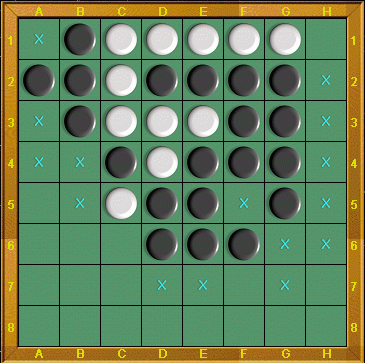
\includegraphics[width=6cm]{Pic/othello}
  \qquad
  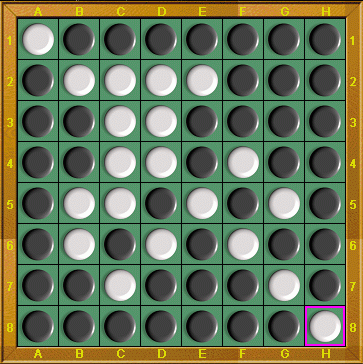
\includegraphics[width=6cm]{Pic/othello2}
  \caption{Othello Game}
  \label{fig:othello}
\end{figure}

You can refer to \url{http://www.tothello.com/html/guideline_of_reversed_othello.html} for more information of guideline, meanwhile, you can download the software to have a try from \url{http://www.tothello.com/html/download.html}. The game installer \texttt{tothello\_trial\_setup.exe} can also be found in the current folder.



\section{Tasks}
\begin{enumerate}

\item In order to reduce the complexity of the game, we think the board is $6\times 6$.

\item There are several evaluation functions that involve many aspects, you can turn to \url{http://blog.sina.com.cn/s/blog_53ebdba00100cpy2.html} for help. In order to reduce the difficulty of the task, I have gaven you some hints of evaluation function in the file \texttt{Heuristic Function for Reversi (Othello).cpp}.

\item Please choose an appropriate evaluation function and use min-max and $\alpha-\beta$ prunning to implement the Othello game. The framework file you can refer to is \texttt{Othello.cpp}. Of course, I wish your program can beat the computer.

\item Write the related codes and take a screenshot of the running results in the file named \textsf{E06\_YourNumber.pdf}, and send it to \textsf{ai\_201901@formail.comhh}
\end{enumerate}

\section{Codes}
%\lstset{
%	numbers=left,   %添加代码的编号,在左侧
%	basicsytle=\ttfamily,   %字母使用打字机字族
%	language=C++  %高亮C++代码
%}

\begin{lstlisting}[language=C++]
int Othello::Judge(Othello *board, enum Option player){
    int value=0;
    Stable(board);
		
    int x = 0, y = 0, i = 0, j = 0, k = 0,
    my_tiles = 0, opp_tiles = 0, 
    my_front_tiles = 0, opp_front_tiles = 0;
		
    double p = 0, m = 0, f = 0, d = 0;
		
    int X1[] = {-1, -1, 0, 1, 1, 1, 0, -1};
    int Y1[] = {0, 1, 1, 1, 0, -1, -1, -1};
    int V[6][6] = {
        {15, 2, 6, 6, 3, 15},
        {2, -3, 0, 0, -3, 2},
        {6, 0, -3, -3, 0, 6},
        {6, 0, -3, -3, 0, 6},
        {2, -3, 0, 0, -3, 2},
        {15, 2, 6, 6, 3, 15},
    };

    for(i = 0; i < 6; i++)
        for(j = 0; j < 6; j++)  {
            if(board->cell[i][j].color == player)  {
                d += V[i][j];
                my_tiles++;
            } 
            else if(board->cell[i][j].color == (enum Option) - player){
                d -= V[i][j];
                opp_tiles++;
            }
            if(board->cell[i][j].color != SPACE)   {
                for(k=0; k<8; k++)  {
                    x = i + X1[k]; y = j + Y1[k];
                    if(x >= 0 && x < 6 && y >= 0 && y < 6 &&
                    board->cell[x][y].color == SPACE) {
                        if(board->cell[i][j].color == player)  my_front_tiles++;
                        else opp_front_tiles++;
                        break;
                    }
                }
            }
        }
    if(my_tiles > opp_tiles)
        p = (100.0 * my_tiles) / (my_tiles + opp_tiles);
    else if(my_tiles < opp_tiles)
        p = -(100.0 * opp_tiles) / (my_tiles + opp_tiles);
    else p = 0;
		
    if(my_front_tiles > opp_front_tiles)
        f = -(100.0 * my_front_tiles) / (my_front_tiles + opp_front_tiles);
    else if(my_front_tiles < opp_front_tiles)
        f = (100.0 * opp_front_tiles) / (my_front_tiles + opp_front_tiles);
    else f = 0;
		
    my_tiles = Rule(board, player);
    opp_tiles = Rule(board, (enum Option) - player);
    if(my_tiles > opp_tiles)
        m = (1.0 * 75 * my_tiles)/(my_tiles + opp_tiles);//75=100*6/8
    else if(my_tiles < opp_tiles)
        m = -(1.0 * 75 * opp_tiles)/(my_tiles + opp_tiles);
    else m = 0;
		
    value = (10 * p) + (78.922 * m) + (74.396 * f) + (10 * d);
    return (int)value;
}
\end{lstlisting}

\section{Results}
\begin{figure}[!h]
    \centering
    \includegraphics[width=8cm]{Pic/result.bmp}

\end{figure}
Among them, white chess is the transformed AI and black chess is the original AI.
%\clearpage
%\bibliography{E:/Papers/LiuLab}
%\bibliographystyle{apalike}
\end{document} 
%%% Local Variables:
%%% mode: latex
%%% TeX-master: t
%%% End:
